% Options for packages loaded elsewhere
\PassOptionsToPackage{unicode}{hyperref}
\PassOptionsToPackage{hyphens}{url}
%
\documentclass[
]{article}
\usepackage{amsmath,amssymb}
\usepackage{lmodern}
\usepackage{iftex}
\ifPDFTeX
  \usepackage[T1]{fontenc}
  \usepackage[utf8]{inputenc}
  \usepackage{textcomp} % provide euro and other symbols
\else % if luatex or xetex
  \usepackage{unicode-math}
  \defaultfontfeatures{Scale=MatchLowercase}
  \defaultfontfeatures[\rmfamily]{Ligatures=TeX,Scale=1}
\fi
% Use upquote if available, for straight quotes in verbatim environments
\IfFileExists{upquote.sty}{\usepackage{upquote}}{}
\IfFileExists{microtype.sty}{% use microtype if available
  \usepackage[]{microtype}
  \UseMicrotypeSet[protrusion]{basicmath} % disable protrusion for tt fonts
}{}
\makeatletter
\@ifundefined{KOMAClassName}{% if non-KOMA class
  \IfFileExists{parskip.sty}{%
    \usepackage{parskip}
  }{% else
    \setlength{\parindent}{0pt}
    \setlength{\parskip}{6pt plus 2pt minus 1pt}}
}{% if KOMA class
  \KOMAoptions{parskip=half}}
\makeatother
\usepackage{xcolor}
\IfFileExists{xurl.sty}{\usepackage{xurl}}{} % add URL line breaks if available
\IfFileExists{bookmark.sty}{\usepackage{bookmark}}{\usepackage{hyperref}}
\hypersetup{
  pdftitle={Analytical exercise of building a linear model},
  hidelinks,
  pdfcreator={LaTeX via pandoc}}
\urlstyle{same} % disable monospaced font for URLs
\usepackage[margin=1in]{geometry}
\usepackage{color}
\usepackage{fancyvrb}
\newcommand{\VerbBar}{|}
\newcommand{\VERB}{\Verb[commandchars=\\\{\}]}
\DefineVerbatimEnvironment{Highlighting}{Verbatim}{commandchars=\\\{\}}
% Add ',fontsize=\small' for more characters per line
\usepackage{framed}
\definecolor{shadecolor}{RGB}{248,248,248}
\newenvironment{Shaded}{\begin{snugshade}}{\end{snugshade}}
\newcommand{\AlertTok}[1]{\textcolor[rgb]{0.94,0.16,0.16}{#1}}
\newcommand{\AnnotationTok}[1]{\textcolor[rgb]{0.56,0.35,0.01}{\textbf{\textit{#1}}}}
\newcommand{\AttributeTok}[1]{\textcolor[rgb]{0.77,0.63,0.00}{#1}}
\newcommand{\BaseNTok}[1]{\textcolor[rgb]{0.00,0.00,0.81}{#1}}
\newcommand{\BuiltInTok}[1]{#1}
\newcommand{\CharTok}[1]{\textcolor[rgb]{0.31,0.60,0.02}{#1}}
\newcommand{\CommentTok}[1]{\textcolor[rgb]{0.56,0.35,0.01}{\textit{#1}}}
\newcommand{\CommentVarTok}[1]{\textcolor[rgb]{0.56,0.35,0.01}{\textbf{\textit{#1}}}}
\newcommand{\ConstantTok}[1]{\textcolor[rgb]{0.00,0.00,0.00}{#1}}
\newcommand{\ControlFlowTok}[1]{\textcolor[rgb]{0.13,0.29,0.53}{\textbf{#1}}}
\newcommand{\DataTypeTok}[1]{\textcolor[rgb]{0.13,0.29,0.53}{#1}}
\newcommand{\DecValTok}[1]{\textcolor[rgb]{0.00,0.00,0.81}{#1}}
\newcommand{\DocumentationTok}[1]{\textcolor[rgb]{0.56,0.35,0.01}{\textbf{\textit{#1}}}}
\newcommand{\ErrorTok}[1]{\textcolor[rgb]{0.64,0.00,0.00}{\textbf{#1}}}
\newcommand{\ExtensionTok}[1]{#1}
\newcommand{\FloatTok}[1]{\textcolor[rgb]{0.00,0.00,0.81}{#1}}
\newcommand{\FunctionTok}[1]{\textcolor[rgb]{0.00,0.00,0.00}{#1}}
\newcommand{\ImportTok}[1]{#1}
\newcommand{\InformationTok}[1]{\textcolor[rgb]{0.56,0.35,0.01}{\textbf{\textit{#1}}}}
\newcommand{\KeywordTok}[1]{\textcolor[rgb]{0.13,0.29,0.53}{\textbf{#1}}}
\newcommand{\NormalTok}[1]{#1}
\newcommand{\OperatorTok}[1]{\textcolor[rgb]{0.81,0.36,0.00}{\textbf{#1}}}
\newcommand{\OtherTok}[1]{\textcolor[rgb]{0.56,0.35,0.01}{#1}}
\newcommand{\PreprocessorTok}[1]{\textcolor[rgb]{0.56,0.35,0.01}{\textit{#1}}}
\newcommand{\RegionMarkerTok}[1]{#1}
\newcommand{\SpecialCharTok}[1]{\textcolor[rgb]{0.00,0.00,0.00}{#1}}
\newcommand{\SpecialStringTok}[1]{\textcolor[rgb]{0.31,0.60,0.02}{#1}}
\newcommand{\StringTok}[1]{\textcolor[rgb]{0.31,0.60,0.02}{#1}}
\newcommand{\VariableTok}[1]{\textcolor[rgb]{0.00,0.00,0.00}{#1}}
\newcommand{\VerbatimStringTok}[1]{\textcolor[rgb]{0.31,0.60,0.02}{#1}}
\newcommand{\WarningTok}[1]{\textcolor[rgb]{0.56,0.35,0.01}{\textbf{\textit{#1}}}}
\usepackage{graphicx}
\makeatletter
\def\maxwidth{\ifdim\Gin@nat@width>\linewidth\linewidth\else\Gin@nat@width\fi}
\def\maxheight{\ifdim\Gin@nat@height>\textheight\textheight\else\Gin@nat@height\fi}
\makeatother
% Scale images if necessary, so that they will not overflow the page
% margins by default, and it is still possible to overwrite the defaults
% using explicit options in \includegraphics[width, height, ...]{}
\setkeys{Gin}{width=\maxwidth,height=\maxheight,keepaspectratio}
% Set default figure placement to htbp
\makeatletter
\def\fps@figure{htbp}
\makeatother
\setlength{\emergencystretch}{3em} % prevent overfull lines
\providecommand{\tightlist}{%
  \setlength{\itemsep}{0pt}\setlength{\parskip}{0pt}}
\setcounter{secnumdepth}{-\maxdimen} % remove section numbering
\ifLuaTeX
  \usepackage{selnolig}  % disable illegal ligatures
\fi

\title{Analytical exercise of building a linear model}
\author{}
\date{\vspace{-2.5em}}

\begin{document}
\maketitle

{
\setcounter{tocdepth}{2}
\tableofcontents
}
This document describes the analytical process that was carried out to
build a linear statistical model properly fitted to the data presented.

The data contained in the \texttt{sbp.csv} file contain observations
from 70 patients. Each observation consists of the following variables:

\begin{itemize}
\tightlist
\item
  sbp -- systolic blood pressure in mmHg
\item
  age -- the age of the patient
\item
  gender -- patient's gender
\end{itemize}

The aim of the study is to estimate a linear model explaining the blood
pressure level and to verify the obtained model.

The adopted significance level in statistical tests is 0.05.

Literature: D. G. Kleinbaum, L. L. Kupper, K. E. Muller, A. Nizam, A.
(1998), Applied Regression Analysis and Other Multivariable Methods,
Duxbury Press, North Scituate, MA

\hypertarget{used-libraries}{%
\paragraph{Used libraries}\label{used-libraries}}

\begin{Shaded}
\begin{Highlighting}[]
\FunctionTok{library}\NormalTok{(}\StringTok{"car"}\NormalTok{)}
\FunctionTok{library}\NormalTok{(}\StringTok{"ggplot2"}\NormalTok{)}
\FunctionTok{library}\NormalTok{(}\StringTok{"lmtest"}\NormalTok{)}
\end{Highlighting}
\end{Shaded}

\hypertarget{data-loading-and-initial-analysis}{%
\subsubsection{Data loading and initial
analysis}\label{data-loading-and-initial-analysis}}

\begin{Shaded}
\begin{Highlighting}[]
\NormalTok{df }\OtherTok{\textless{}{-}}  \FunctionTok{read.table}\NormalTok{(}\StringTok{"sbp.csv"}\NormalTok{, }\AttributeTok{header =} \ConstantTok{TRUE}\NormalTok{, }\AttributeTok{sep =} \StringTok{";"}\NormalTok{,}\AttributeTok{dec=}\StringTok{","}\NormalTok{)}
\end{Highlighting}
\end{Shaded}

Descriptive statistics for variables in the dataset:

\begin{Shaded}
\begin{Highlighting}[]
\NormalTok{df}\SpecialCharTok{$}\NormalTok{gender }\OtherTok{\textless{}{-}} \FunctionTok{as.factor}\NormalTok{(df}\SpecialCharTok{$}\NormalTok{gender)}
\FunctionTok{summary}\NormalTok{(df)}
\end{Highlighting}
\end{Shaded}

\begin{verbatim}
##     gender        sbp             age       
##  female:29   Min.   :110.0   Min.   :17.00  
##  male  :41   1st Qu.:135.2   1st Qu.:36.50  
##              Median :149.5   Median :47.00  
##              Mean   :149.7   Mean   :46.16  
##              3rd Qu.:162.0   3rd Qu.:58.50  
##              Max.   :220.0   Max.   :70.00
\end{verbatim}

\hypertarget{linear-model-with-age-variable}{%
\subsection{Linear model with age
variable}\label{linear-model-with-age-variable}}

\hypertarget{estimation-of-model-1}{%
\subsubsection{Estimation of Model 1}\label{estimation-of-model-1}}

\begin{Shaded}
\begin{Highlighting}[]
\NormalTok{m1 }\OtherTok{\textless{}{-}} \FunctionTok{lm}\NormalTok{(sbp }\SpecialCharTok{\textasciitilde{}}\NormalTok{ age, }\AttributeTok{data =}\NormalTok{ df)}
\FunctionTok{summary}\NormalTok{(m1)}
\end{Highlighting}
\end{Shaded}

\begin{verbatim}
## 
## Call:
## lm(formula = sbp ~ age, data = df)
## 
## Residuals:
##     Min      1Q  Median      3Q     Max 
## -27.742  -8.450   1.194   7.322  69.425 
## 
## Coefficients:
##             Estimate Std. Error t value Pr(>|t|)    
## (Intercept) 104.1781     5.4228  19.211  < 2e-16 ***
## age           0.9872     0.1118   8.827 6.93e-13 ***
## ---
## Signif. codes:  0 '***' 0.001 '**' 0.01 '*' 0.05 '.' 0.1 ' ' 1
## 
## Residual standard error: 13.91 on 68 degrees of freedom
## Multiple R-squared:  0.534,  Adjusted R-squared:  0.5271 
## F-statistic: 77.92 on 1 and 68 DF,  p-value: 6.925e-13
\end{verbatim}

Model 1: \(y_{i} = 104.1781 + 0.9872x_{1} + e_{i}\)

Interpretation of the model parameter significance tests:

\begin{itemize}
\item
  For Wald's test of total significance of parameters (F-statistic)
  \texttt{p-value\ \textless{}\ 0.05}, therefore we reject the null
  hypothesis that all model parameters are irrelevant. There is at least
  one parameter that significantly influences the model's variability.
\item
  For t-student tests of the significance of a single parameter for both
  the parameter \texttt{b0} and\texttt{b1}
  \texttt{p-value\ \textless{}\ 0.05}, therefore we reject the null
  hypotheses about the irrelevance of the parameters for the model. Both
  parameters significantly affect the variability of the model.
\end{itemize}

The model explains the variability of the phenomenon in 53\%.

\hypertarget{model-visualization}{%
\subparagraph{Model visualization}\label{model-visualization}}

\begin{Shaded}
\begin{Highlighting}[]
\NormalTok{wykres }\OtherTok{\textless{}{-}} \FunctionTok{ggplot}\NormalTok{() }\SpecialCharTok{+}
  \FunctionTok{ggtitle}\NormalTok{(}\StringTok{"Linear model sbp = b0 + b1 * age"}\NormalTok{) }\SpecialCharTok{+}
  \FunctionTok{geom\_point}\NormalTok{(}\FunctionTok{aes}\NormalTok{(df}\SpecialCharTok{$}\NormalTok{age, df}\SpecialCharTok{$}\NormalTok{sbp)) }\SpecialCharTok{+}
  \FunctionTok{geom\_line}\NormalTok{(}\FunctionTok{aes}\NormalTok{(m1}\SpecialCharTok{$}\NormalTok{model}\SpecialCharTok{$}\NormalTok{age, m1}\SpecialCharTok{$}\NormalTok{fitted.values), }\AttributeTok{color =} \StringTok{"green3"}\NormalTok{) }\SpecialCharTok{+}
  \FunctionTok{xlab}\NormalTok{(}\StringTok{"age"}\NormalTok{)}\SpecialCharTok{+}
  \FunctionTok{ylab}\NormalTok{(}\StringTok{"systolic blood pressure"}\NormalTok{) }\SpecialCharTok{+}
  \FunctionTok{theme\_classic}\NormalTok{()}
\FunctionTok{plot}\NormalTok{(wykres)}
\end{Highlighting}
\end{Shaded}

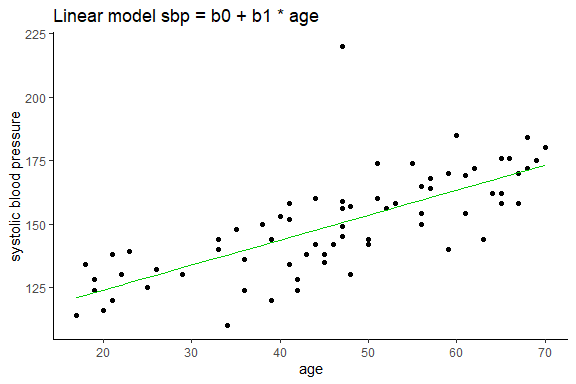
\includegraphics{linear_model_exercise_files/figure-latex/unnamed-chunk-5-1.pdf}

\hypertarget{verification-of-the-model-1-assumptions}{%
\subsubsection{Verification of the Model 1
assumptions}\label{verification-of-the-model-1-assumptions}}

Before performing the statistical tests, you can look at the three
graphs below to roughly determine the characteristics of the model.

\begin{Shaded}
\begin{Highlighting}[]
\FunctionTok{plot}\NormalTok{(m1, }\AttributeTok{which =} \DecValTok{1}\SpecialCharTok{:}\DecValTok{3}\NormalTok{)}
\end{Highlighting}
\end{Shaded}

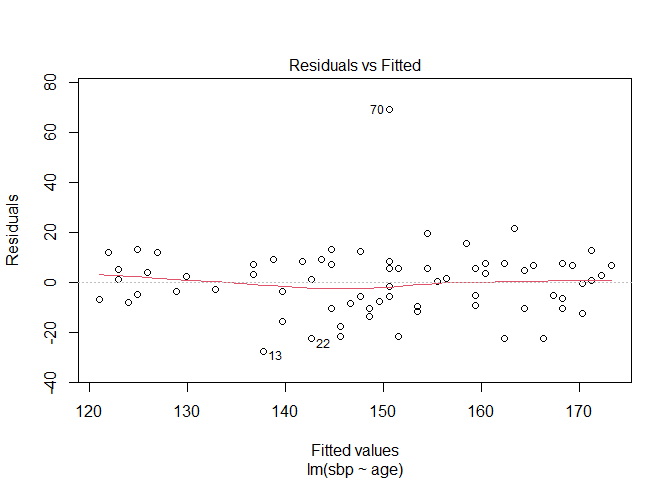
\includegraphics{linear_model_exercise_files/figure-latex/unnamed-chunk-6-1.pdf}
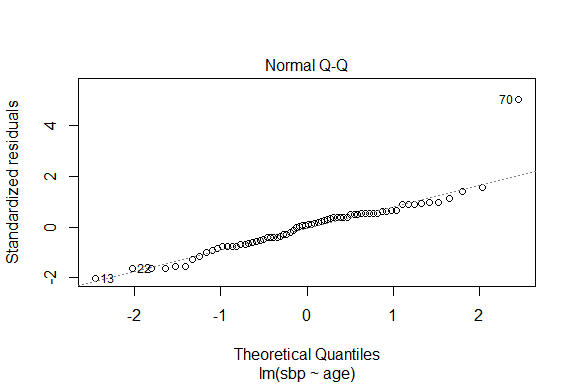
\includegraphics{linear_model_exercise_files/figure-latex/unnamed-chunk-6-2.pdf}
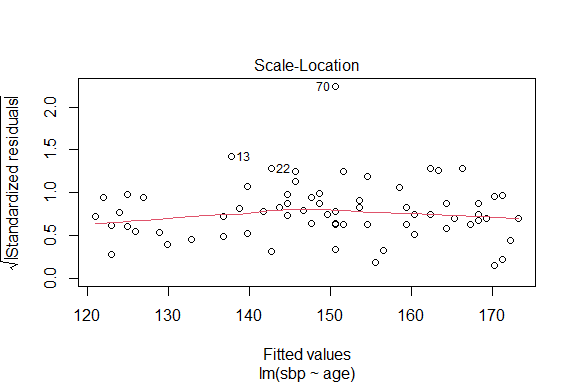
\includegraphics{linear_model_exercise_files/figure-latex/unnamed-chunk-6-3.pdf}

From the graphs it can be concluded that the mean value of the residuals
is close to 0, which means that the assumption of a linear relationship
was valid. Moreover, the variance of the random term is constant (there
is homoscedasticity). There is an outlier, denoted as observation number
70, which distorts the estimate and rules out the normality of the
distribution of the residuals.

\hypertarget{statistical-tests}{%
\paragraph{Statistical tests}\label{statistical-tests}}

\hypertarget{shapiro-wilk-normality-test-for-residuals}{%
\subparagraph{Shapiro-Wilk normality test for
residuals}\label{shapiro-wilk-normality-test-for-residuals}}

\begin{Shaded}
\begin{Highlighting}[]
\FunctionTok{shapiro.test}\NormalTok{(m1}\SpecialCharTok{$}\NormalTok{residuals)}
\end{Highlighting}
\end{Shaded}

\begin{verbatim}
## 
##  Shapiro-Wilk normality test
## 
## data:  m1$residuals
## W = 0.87623, p-value = 5.035e-06
\end{verbatim}

\textbf{Conclusion}: \texttt{p-value\ \textless{}\ 0.05}, we reject the
null hypothesis of normal residual distribution.

\hypertarget{breusch-pagan-test-for-heteroskedasticity}{%
\subparagraph{Breusch-Pagan test for
heteroskedasticity}\label{breusch-pagan-test-for-heteroskedasticity}}

\begin{Shaded}
\begin{Highlighting}[]
\FunctionTok{bptest}\NormalTok{(m1)}
\end{Highlighting}
\end{Shaded}

\begin{verbatim}
## 
##  studentized Breusch-Pagan test
## 
## data:  m1
## BP = 0.013838, df = 1, p-value = 0.9064
\end{verbatim}

\textbf{Conclusion}: \texttt{p-value\ \textgreater{}\ 0.05}, no grounds
for rejecting the null hypothesis, the residuals are distributed with
equal variance.

\hypertarget{durbin-watson-test-for-autocorrelation}{%
\subparagraph{Durbin-Watson test for
autocorrelation}\label{durbin-watson-test-for-autocorrelation}}

\begin{Shaded}
\begin{Highlighting}[]
\FunctionTok{dwtest}\NormalTok{(m1, }\AttributeTok{order.by =} \SpecialCharTok{\textasciitilde{}}\NormalTok{age, }\AttributeTok{data =}\NormalTok{ df)}
\end{Highlighting}
\end{Shaded}

\begin{verbatim}
## 
##  Durbin-Watson test
## 
## data:  m1
## DW = 2.3105, p-value = 0.8826
## alternative hypothesis: true autocorrelation is greater than 0
\end{verbatim}

\textbf{Conclusion}: \texttt{p-value\ \textgreater{}\ 0.05}, no grounds
for rejecting the null hypothesis, the residuals are not autocorrelated.

\hypertarget{harvey-collier-test-for-linearity}{%
\subparagraph{Harvey-Collier test for
linearity}\label{harvey-collier-test-for-linearity}}

\begin{Shaded}
\begin{Highlighting}[]
\FunctionTok{harvtest}\NormalTok{(m1, }\AttributeTok{order.by =} \SpecialCharTok{\textasciitilde{}}\NormalTok{age, }\AttributeTok{data =}\NormalTok{ df)}
\end{Highlighting}
\end{Shaded}

\begin{verbatim}
## 
##  Harvey-Collier test
## 
## data:  m1
## HC = 0.52181, df = 67, p-value = 0.6035
\end{verbatim}

\textbf{Conclusion}: \texttt{p-value\ \textgreater{}\ 0.05}, no grounds
for rejecting the null hypothesis, the regression is correctly modeled
as linear.

\hypertarget{detecting-influential-observations}{%
\subparagraph{Detecting influential
observations}\label{detecting-influential-observations}}

The following graphs show the assessment of the impact of individual
observations on the structural parameters of Model 1 using measures:
Cook's distance, leverage influence indicator.

\begin{Shaded}
\begin{Highlighting}[]
\FunctionTok{plot}\NormalTok{(m1, }\AttributeTok{which =} \DecValTok{4}\SpecialCharTok{:}\DecValTok{5}\NormalTok{)}
\end{Highlighting}
\end{Shaded}

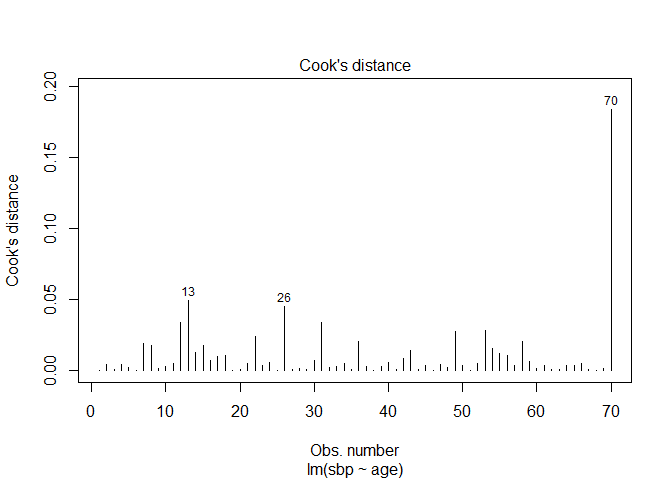
\includegraphics{linear_model_exercise_files/figure-latex/unnamed-chunk-11-1.pdf}
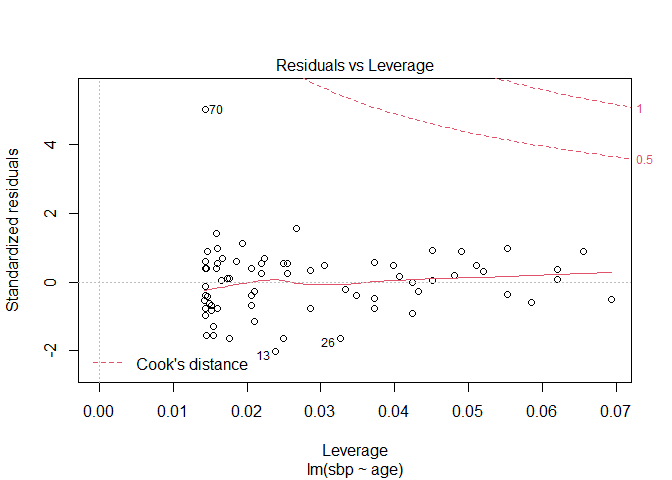
\includegraphics{linear_model_exercise_files/figure-latex/unnamed-chunk-11-2.pdf}

\hypertarget{estimation-of-model-2}{%
\subsubsection{Estimation of Model 2}\label{estimation-of-model-2}}

The model below was estimated after discarding atypical observation
number 70.

\begin{Shaded}
\begin{Highlighting}[]
\NormalTok{m2 }\OtherTok{\textless{}{-}} \FunctionTok{lm}\NormalTok{(sbp }\SpecialCharTok{\textasciitilde{}}\NormalTok{ age, }\AttributeTok{data =}\NormalTok{ df, }\AttributeTok{subset =} \DecValTok{1}\SpecialCharTok{:}\DecValTok{69}\NormalTok{)}
\FunctionTok{summary}\NormalTok{(m2)}
\end{Highlighting}
\end{Shaded}

\begin{verbatim}
## 
## Call:
## lm(formula = sbp ~ age, data = df, subset = 1:69)
## 
## Residuals:
##     Min      1Q  Median      3Q     Max 
## -26.782  -7.632   1.968   8.201  22.651 
## 
## Coefficients:
##              Estimate Std. Error t value Pr(>|t|)    
## (Intercept) 103.34905    4.33190   23.86   <2e-16 ***
## age           0.98333    0.08929   11.01   <2e-16 ***
## ---
## Signif. codes:  0 '***' 0.001 '**' 0.01 '*' 0.05 '.' 0.1 ' ' 1
## 
## Residual standard error: 11.1 on 67 degrees of freedom
## Multiple R-squared:  0.6441, Adjusted R-squared:  0.6388 
## F-statistic: 121.3 on 1 and 67 DF,  p-value: < 2.2e-16
\end{verbatim}

Model 2: \(y_{i} = 103.3491 + 0.9833x_{1} + e_{i}\)

\textbf{Findings}: The standard deviation of residuals decreased and the
degree of explanation of variability by the model increased to 63\%.

The chart below shows a comparison between model 1 and model 2, before
and after the rejection of outliers.

\begin{Shaded}
\begin{Highlighting}[]
\NormalTok{wykres }\OtherTok{\textless{}{-}} \FunctionTok{ggplot}\NormalTok{() }\SpecialCharTok{+}
  \FunctionTok{ggtitle}\NormalTok{(}\StringTok{"Linear models comparison"}\NormalTok{, }
          \AttributeTok{subtitle=} \StringTok{"          green line {-} model for the entire set, }
\StringTok{          orange line {-} model after discarding outliers"}\NormalTok{) }\SpecialCharTok{+}
  \FunctionTok{geom\_point}\NormalTok{(}\FunctionTok{aes}\NormalTok{(df}\SpecialCharTok{$}\NormalTok{age, df}\SpecialCharTok{$}\NormalTok{sbp)) }\SpecialCharTok{+}
  \FunctionTok{geom\_line}\NormalTok{(}\FunctionTok{aes}\NormalTok{(m1}\SpecialCharTok{$}\NormalTok{model}\SpecialCharTok{$}\NormalTok{age, m1}\SpecialCharTok{$}\NormalTok{fitted.values), }\AttributeTok{color =} \StringTok{"green3"}\NormalTok{) }\SpecialCharTok{+}
  \FunctionTok{geom\_line}\NormalTok{(}\FunctionTok{aes}\NormalTok{(m2}\SpecialCharTok{$}\NormalTok{model}\SpecialCharTok{$}\NormalTok{age, m2}\SpecialCharTok{$}\NormalTok{fitted.values), }\AttributeTok{color =} \StringTok{"darkorange"}\NormalTok{) }\SpecialCharTok{+}
  \FunctionTok{xlab}\NormalTok{(}\StringTok{"age"}\NormalTok{)}\SpecialCharTok{+}
  \FunctionTok{ylab}\NormalTok{(}\StringTok{"systolic blood pressure"}\NormalTok{) }\SpecialCharTok{+}
  \FunctionTok{theme\_classic}\NormalTok{()}
\FunctionTok{plot}\NormalTok{(wykres)}
\end{Highlighting}
\end{Shaded}

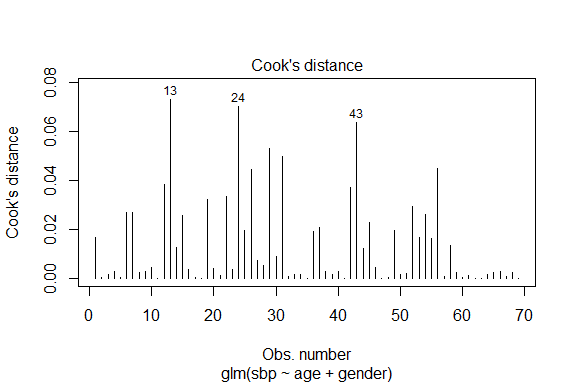
\includegraphics{linear_model_exercise_files/figure-latex/unnamed-chunk-13-1.pdf}

\hypertarget{verification-of-the-model-2-assumptions}{%
\subsubsection{Verification of the Model 2
assumptions}\label{verification-of-the-model-2-assumptions}}

Diagnostic charts for Model 2.

\begin{Shaded}
\begin{Highlighting}[]
\FunctionTok{plot}\NormalTok{(m2)}
\end{Highlighting}
\end{Shaded}

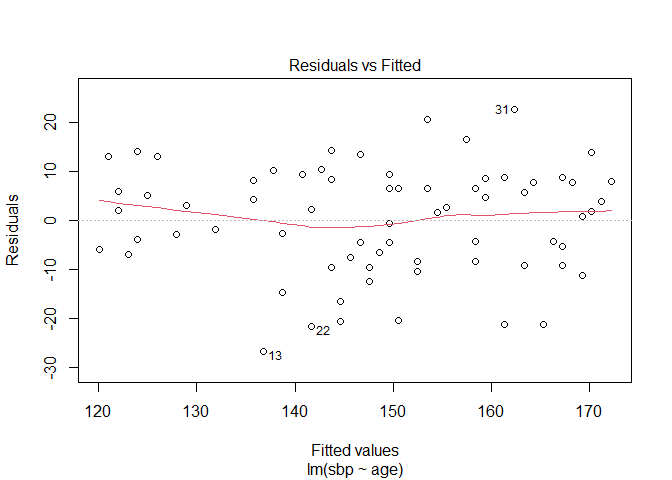
\includegraphics{linear_model_exercise_files/figure-latex/unnamed-chunk-14-1.pdf}
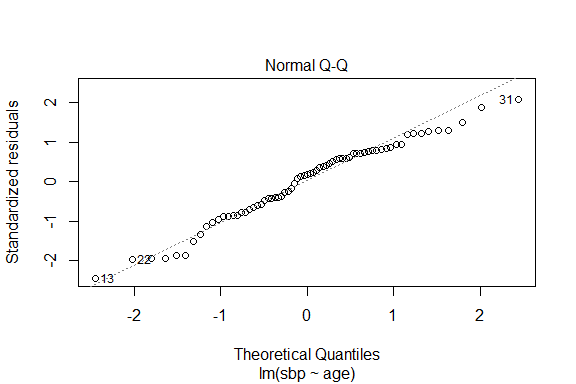
\includegraphics{linear_model_exercise_files/figure-latex/unnamed-chunk-14-2.pdf}
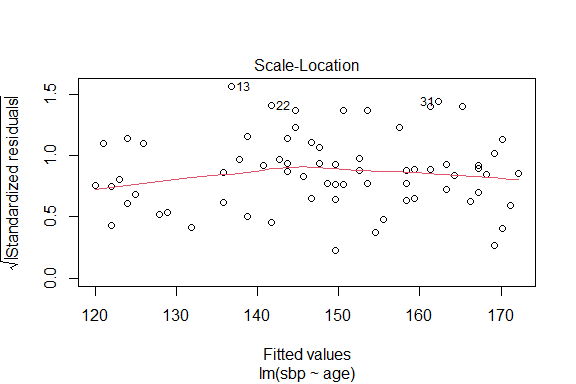
\includegraphics{linear_model_exercise_files/figure-latex/unnamed-chunk-14-3.pdf}
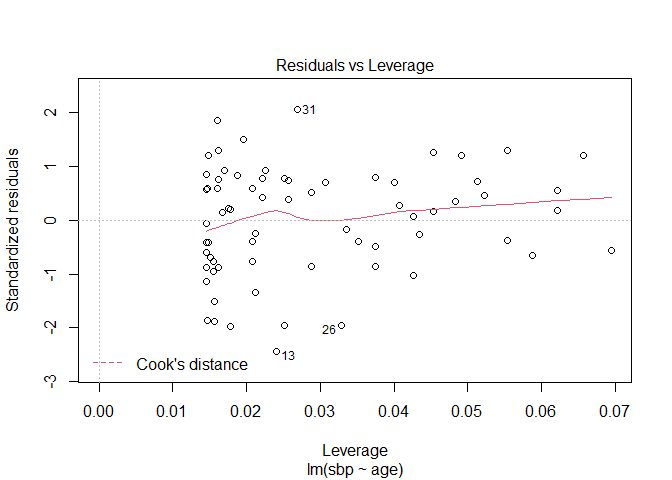
\includegraphics{linear_model_exercise_files/figure-latex/unnamed-chunk-14-4.pdf}

There are only slight changes in the charts. The fit of the values in
the Normal Q-Q plot has improved.

\hypertarget{statistical-tests-1}{%
\paragraph{Statistical tests}\label{statistical-tests-1}}

\hypertarget{shapiro-wilk-normality-test-for-residuals-1}{%
\subparagraph{Shapiro-Wilk normality test for
residuals}\label{shapiro-wilk-normality-test-for-residuals-1}}

\begin{Shaded}
\begin{Highlighting}[]
\FunctionTok{shapiro.test}\NormalTok{(m2}\SpecialCharTok{$}\NormalTok{residuals)}
\end{Highlighting}
\end{Shaded}

\begin{verbatim}
## 
##  Shapiro-Wilk normality test
## 
## data:  m2$residuals
## W = 0.97263, p-value = 0.134
\end{verbatim}

\textbf{Conclusion}: \texttt{p-value\ \textgreater{}\ 0.05}, no grounds
for rejecting the null hypothesis, the residuals are normally
distributed.

\hypertarget{breusch-pagan-test-for-heteroskedasticity-1}{%
\subparagraph{Breusch-Pagan test for
heteroskedasticity}\label{breusch-pagan-test-for-heteroskedasticity-1}}

\begin{Shaded}
\begin{Highlighting}[]
\FunctionTok{bptest}\NormalTok{(m2)}
\end{Highlighting}
\end{Shaded}

\begin{verbatim}
## 
##  studentized Breusch-Pagan test
## 
## data:  m2
## BP = 0.060841, df = 1, p-value = 0.8052
\end{verbatim}

\textbf{Conclusion}: \texttt{p-value\ \textgreater{}\ 0.05}, no grounds
for rejecting the null hypothesis, the residuals are distributed with
equal variance.

\hypertarget{durbin-watson-test-for-autocorrelation-1}{%
\subparagraph{Durbin-Watson test for
autocorrelation}\label{durbin-watson-test-for-autocorrelation-1}}

\begin{Shaded}
\begin{Highlighting}[]
\FunctionTok{dwtest}\NormalTok{(m2, }\AttributeTok{order.by =} \SpecialCharTok{\textasciitilde{}}\NormalTok{age, }\AttributeTok{data =}\NormalTok{ df[}\DecValTok{1}\SpecialCharTok{:}\DecValTok{69}\NormalTok{,])}
\end{Highlighting}
\end{Shaded}

\begin{verbatim}
## 
##  Durbin-Watson test
## 
## data:  m2
## DW = 2.1141, p-value = 0.6373
## alternative hypothesis: true autocorrelation is greater than 0
\end{verbatim}

\textbf{Conclusion}: \texttt{p-value\ \textgreater{}\ 0.05}, no grounds
for rejecting the null hypothesis, the residuals are not autocorrelated.

\hypertarget{harvey-collier-test-for-linearity-1}{%
\subparagraph{Harvey-Collier test for
linearity}\label{harvey-collier-test-for-linearity-1}}

\begin{Shaded}
\begin{Highlighting}[]
\FunctionTok{harvtest}\NormalTok{(m2, }\AttributeTok{order.by =} \SpecialCharTok{\textasciitilde{}}\NormalTok{age, }\AttributeTok{data =}\NormalTok{ df[}\DecValTok{1}\SpecialCharTok{:}\DecValTok{69}\NormalTok{,])}
\end{Highlighting}
\end{Shaded}

\begin{verbatim}
## 
##  Harvey-Collier test
## 
## data:  m2
## HC = 0.79742, df = 66, p-value = 0.4281
\end{verbatim}

\textbf{Conclusion}: \texttt{p-value\ \textgreater{}\ 0.05}, no grounds
for rejecting the null hypothesis, the regression is correctly modeled
as linear.

\hypertarget{bonferroni-outlier-test}{%
\subparagraph{Bonferroni Outlier Test}\label{bonferroni-outlier-test}}

\begin{Shaded}
\begin{Highlighting}[]
\FunctionTok{outlierTest}\NormalTok{(m1, }\AttributeTok{n.max =} \ConstantTok{Inf}\NormalTok{)}
\end{Highlighting}
\end{Shaded}

\begin{verbatim}
##    rstudent unadjusted p-value Bonferroni p
## 70 6.297744         2.6747e-08   1.8723e-06
\end{verbatim}

\begin{Shaded}
\begin{Highlighting}[]
\FunctionTok{outlierTest}\NormalTok{(m2, }\AttributeTok{n.max =} \ConstantTok{Inf}\NormalTok{)}
\end{Highlighting}
\end{Shaded}

\begin{verbatim}
## No Studentized residuals with Bonferroni p < 0.05
## Largest |rstudent|:
##     rstudent unadjusted p-value Bonferroni p
## 13 -2.538813           0.013489      0.93071
\end{verbatim}

Based on the Bonferroni test, it can be seen that after excluding
outlier number 70, there is no need to remove other observations.

\hypertarget{linear-model-with-age-and-gender-variables}{%
\subsection{Linear model with age and gender
variables}\label{linear-model-with-age-and-gender-variables}}

\hypertarget{estimation-of-model-3}{%
\subsubsection{Estimation of Model 3}\label{estimation-of-model-3}}

\begin{Shaded}
\begin{Highlighting}[]
\NormalTok{m3 }\OtherTok{\textless{}{-}} \FunctionTok{lm}\NormalTok{(sbp }\SpecialCharTok{\textasciitilde{}}\NormalTok{ age }\SpecialCharTok{+}\NormalTok{ gender, }\AttributeTok{data =}\NormalTok{ df, }\AttributeTok{subset =} \DecValTok{1}\SpecialCharTok{:}\DecValTok{69}\NormalTok{)}
\FunctionTok{summary}\NormalTok{(m3)}
\end{Highlighting}
\end{Shaded}

\begin{verbatim}
## 
## Call:
## lm(formula = sbp ~ age + gender, data = df, subset = 1:69)
## 
## Residuals:
##     Min      1Q  Median      3Q     Max 
## -20.705  -3.299   1.248   4.325  21.160 
## 
## Coefficients:
##             Estimate Std. Error t value Pr(>|t|)    
## (Intercept) 96.77353    3.62085  26.727  < 2e-16 ***
## age          0.95606    0.07153  13.366  < 2e-16 ***
## gendermale  13.51345    2.16932   6.229  3.7e-08 ***
## ---
## Signif. codes:  0 '***' 0.001 '**' 0.01 '*' 0.05 '.' 0.1 ' ' 1
## 
## Residual standard error: 8.878 on 66 degrees of freedom
## Multiple R-squared:  0.7759, Adjusted R-squared:  0.7691 
## F-statistic: 114.2 on 2 and 66 DF,  p-value: < 2.2e-16
\end{verbatim}

Model 3: \(y_{i} = 96.7735 + 0.9872x_{1} + 13.5135x_{2} + e_{i}\)

\textbf{Findings}: The standard deviation of residuals decreased further
and the degree of explanation of variability by the model increased to
77\%.

Shown below in the graph is Model 3 for men and women.

\begin{Shaded}
\begin{Highlighting}[]
\FunctionTok{ggplot}\NormalTok{() }\SpecialCharTok{+}
  \FunctionTok{ggtitle}\NormalTok{(}\StringTok{"Linear model sbp = b0 + b1 * age + b2 * gender"}\NormalTok{, }
          \AttributeTok{subtitle=} \StringTok{"          blue {-} male}
\StringTok{          red {-} female"}\NormalTok{) }\SpecialCharTok{+}
  \FunctionTok{geom\_point}\NormalTok{(}\FunctionTok{aes}\NormalTok{(m3}\SpecialCharTok{$}\NormalTok{model[m3}\SpecialCharTok{$}\NormalTok{model}\SpecialCharTok{$}\NormalTok{gender}\SpecialCharTok{==}\StringTok{"male"}\NormalTok{,]}\SpecialCharTok{$}\NormalTok{age, m3}\SpecialCharTok{$}\NormalTok{model[m3}\SpecialCharTok{$}\NormalTok{model}\SpecialCharTok{$}\NormalTok{gender}\SpecialCharTok{==}\StringTok{"male"}\NormalTok{,]}\SpecialCharTok{$}\NormalTok{sbp), }\AttributeTok{color =} \StringTok{"blue"}\NormalTok{) }\SpecialCharTok{+}
  \FunctionTok{geom\_point}\NormalTok{(}\FunctionTok{aes}\NormalTok{(m3}\SpecialCharTok{$}\NormalTok{model[m3}\SpecialCharTok{$}\NormalTok{model}\SpecialCharTok{$}\NormalTok{gender}\SpecialCharTok{==}\StringTok{"female"}\NormalTok{,]}\SpecialCharTok{$}\NormalTok{age, m3}\SpecialCharTok{$}\NormalTok{model[m3}\SpecialCharTok{$}\NormalTok{model}\SpecialCharTok{$}\NormalTok{gender}\SpecialCharTok{==}\StringTok{"female"}\NormalTok{,]}\SpecialCharTok{$}\NormalTok{sbp), }\AttributeTok{color =} \StringTok{"red"}\NormalTok{) }\SpecialCharTok{+}
  \FunctionTok{geom\_line}\NormalTok{(}\FunctionTok{aes}\NormalTok{(m3}\SpecialCharTok{$}\NormalTok{model[m3}\SpecialCharTok{$}\NormalTok{model}\SpecialCharTok{$}\NormalTok{gender}\SpecialCharTok{==}\StringTok{"male"}\NormalTok{,]}\SpecialCharTok{$}\NormalTok{age, }\FunctionTok{predict}\NormalTok{(m3, }\FunctionTok{data.frame}\NormalTok{(}\AttributeTok{age =}\NormalTok{ m3}\SpecialCharTok{$}\NormalTok{model[m3}\SpecialCharTok{$}\NormalTok{model}\SpecialCharTok{$}\NormalTok{gender}\SpecialCharTok{==}\StringTok{"male"}\NormalTok{,]}\SpecialCharTok{$}\NormalTok{age, }\AttributeTok{gender =}\StringTok{"male"}\NormalTok{))), }\AttributeTok{color =} \StringTok{"blue"}\NormalTok{) }\SpecialCharTok{+}
  \FunctionTok{geom\_line}\NormalTok{(}\FunctionTok{aes}\NormalTok{(m3}\SpecialCharTok{$}\NormalTok{model[m3}\SpecialCharTok{$}\NormalTok{model}\SpecialCharTok{$}\NormalTok{gender}\SpecialCharTok{==}\StringTok{"female"}\NormalTok{,]}\SpecialCharTok{$}\NormalTok{age, }\FunctionTok{predict}\NormalTok{(m3, }\FunctionTok{data.frame}\NormalTok{(}\AttributeTok{age =}\NormalTok{ m3}\SpecialCharTok{$}\NormalTok{model[m3}\SpecialCharTok{$}\NormalTok{model}\SpecialCharTok{$}\NormalTok{gender}\SpecialCharTok{==}\StringTok{"female"}\NormalTok{,]}\SpecialCharTok{$}\NormalTok{age, }\AttributeTok{gender =}\StringTok{"female"}\NormalTok{))), }\AttributeTok{color =} \StringTok{"red"}\NormalTok{) }\SpecialCharTok{+}
  \FunctionTok{xlab}\NormalTok{(}\StringTok{"age"}\NormalTok{)}\SpecialCharTok{+}
  \FunctionTok{ylab}\NormalTok{(}\StringTok{"systolic blood pressure"}\NormalTok{) }\SpecialCharTok{+}
  \FunctionTok{theme\_classic}\NormalTok{()}
\end{Highlighting}
\end{Shaded}

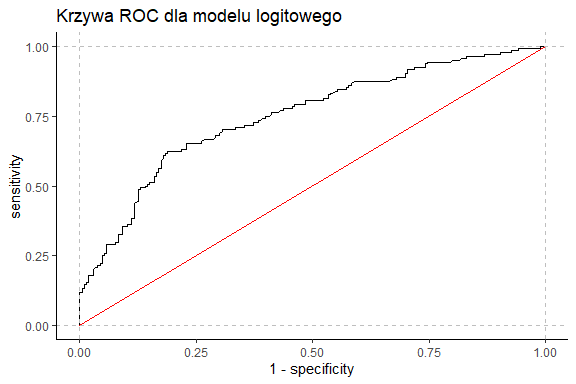
\includegraphics{linear_model_exercise_files/figure-latex/unnamed-chunk-21-1.pdf}

\textbf{Interpretation of Model 3 parameters}

The constant term \texttt{b0\ =\ 96.7} in this model is not interpreted
as the study did not include infants or children.

For \texttt{b1\ =\ 0.9561} with the variable\texttt{age} If the age
increases by 1 year, the blood pressure will increase by an average of
0.9561 mmHg for people of the same sex, ceteris paribus.

For \texttt{b2\ =\ 13.5134} with the variable\texttt{gender} The blood
pressure of men is on average 13.51 mmHg higher than that of women of
the same age, ceteris paribus.

\hypertarget{verification-of-the-model-3-assumptions}{%
\subsubsection{Verification of the Model 3
assumptions}\label{verification-of-the-model-3-assumptions}}

Checking whether explanatory variables are not collinear.

\begin{Shaded}
\begin{Highlighting}[]
\FunctionTok{vif}\NormalTok{(m3)}
\end{Highlighting}
\end{Shaded}

\begin{verbatim}
##      age   gender 
## 1.003759 1.003759
\end{verbatim}

Diagnostic charts for Model 3

\begin{Shaded}
\begin{Highlighting}[]
\FunctionTok{plot}\NormalTok{(m3)}
\end{Highlighting}
\end{Shaded}

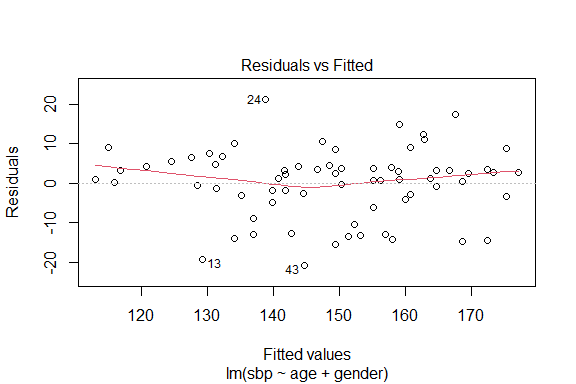
\includegraphics{linear_model_exercise_files/figure-latex/unnamed-chunk-23-1.pdf}
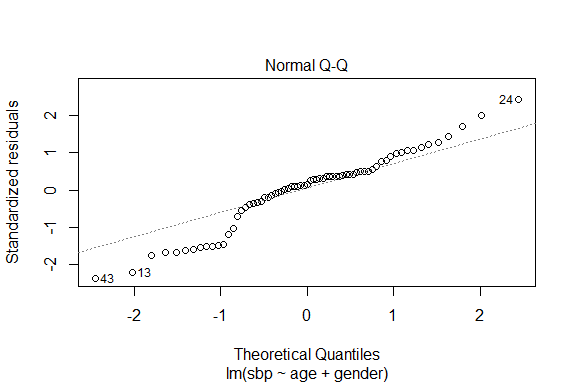
\includegraphics{linear_model_exercise_files/figure-latex/unnamed-chunk-23-2.pdf}
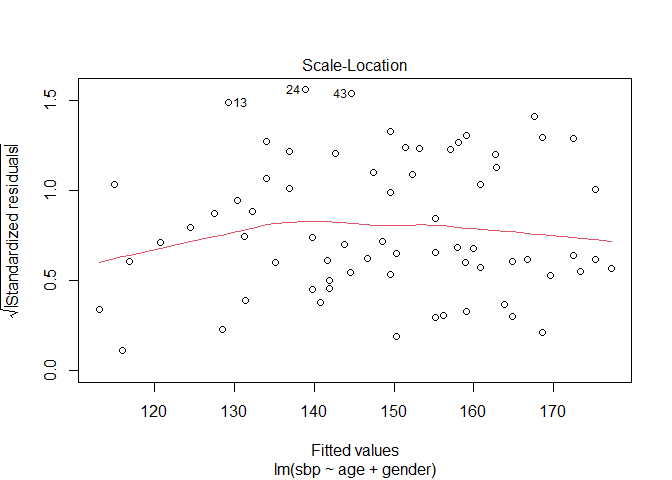
\includegraphics{linear_model_exercise_files/figure-latex/unnamed-chunk-23-3.pdf}
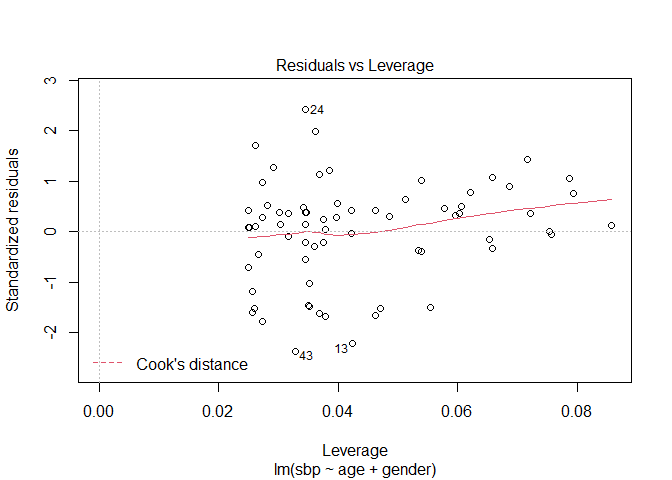
\includegraphics{linear_model_exercise_files/figure-latex/unnamed-chunk-23-4.pdf}

\hypertarget{statistical-tests-2}{%
\paragraph{Statistical tests}\label{statistical-tests-2}}

\hypertarget{shapiro-wilk-normality-test-for-residuals-2}{%
\subparagraph{Shapiro-Wilk normality test for
residuals}\label{shapiro-wilk-normality-test-for-residuals-2}}

\begin{Shaded}
\begin{Highlighting}[]
\FunctionTok{shapiro.test}\NormalTok{(m3}\SpecialCharTok{$}\NormalTok{residuals)}
\end{Highlighting}
\end{Shaded}

\begin{verbatim}
## 
##  Shapiro-Wilk normality test
## 
## data:  m3$residuals
## W = 0.95573, p-value = 0.01567
\end{verbatim}

\textbf{Conclusion}: \texttt{p-value\ \textless{}\ 0.05}, we reject the
null hypothesis of normal residual distribution.

\hypertarget{breusch-pagan-test-for-heteroskedasticity-2}{%
\subparagraph{Breusch-Pagan test for
heteroskedasticity}\label{breusch-pagan-test-for-heteroskedasticity-2}}

\begin{Shaded}
\begin{Highlighting}[]
\FunctionTok{bptest}\NormalTok{(m3)}
\end{Highlighting}
\end{Shaded}

\begin{verbatim}
## 
##  studentized Breusch-Pagan test
## 
## data:  m3
## BP = 0.66927, df = 2, p-value = 0.7156
\end{verbatim}

\textbf{Conclusion}: \texttt{p-value\ \textgreater{}\ 0.05}, no grounds
for rejecting the null hypothesis, the residuals are distributed with
equal variance.

\hypertarget{durbin-watson-test-for-autocorrelation-2}{%
\subparagraph{Durbin-Watson test for
autocorrelation}\label{durbin-watson-test-for-autocorrelation-2}}

\begin{Shaded}
\begin{Highlighting}[]
\FunctionTok{dwtest}\NormalTok{(m3, }\AttributeTok{order.by =} \SpecialCharTok{\textasciitilde{}}\NormalTok{age, }\AttributeTok{data =}\NormalTok{ df[}\DecValTok{1}\SpecialCharTok{:}\DecValTok{69}\NormalTok{,])}
\end{Highlighting}
\end{Shaded}

\begin{verbatim}
## 
##  Durbin-Watson test
## 
## data:  m3
## DW = 2.2791, p-value = 0.8545
## alternative hypothesis: true autocorrelation is greater than 0
\end{verbatim}

\textbf{Conclusion}: \texttt{p-value\ \textgreater{}\ 0.05}, no grounds
for rejecting the null hypothesis, the residuals are not autocorrelated.

\hypertarget{harvey-collier-test-for-linearity-2}{%
\subparagraph{Harvey-Collier test for
linearity}\label{harvey-collier-test-for-linearity-2}}

\begin{Shaded}
\begin{Highlighting}[]
\FunctionTok{harvtest}\NormalTok{(m3, }\AttributeTok{order.by =} \SpecialCharTok{\textasciitilde{}}\NormalTok{age, }\AttributeTok{data =}\NormalTok{ df[}\DecValTok{1}\SpecialCharTok{:}\DecValTok{69}\NormalTok{,])}
\end{Highlighting}
\end{Shaded}

\begin{verbatim}
## 
##  Harvey-Collier test
## 
## data:  m3
## HC = 1.2289, df = 65, p-value = 0.2235
\end{verbatim}

\textbf{Conclusion}: \texttt{p-value\ \textgreater{}\ 0.05}, no grounds
for rejecting the null hypothesis, the regression is correctly modeled
as linear.

\hypertarget{summary}{%
\subsection{Summary}\label{summary}}

In model 2, the residuals are normally distributed, but the model
explains only 64\% of the variation in blood pressure. When the gender
variable was added, the fit of the model improved: the standard
deviation of the residuals decreased, Model 3 explained 77\% of the
blood pressure development, but the residuals did not have a normal
distribution. Another form of model is needed.

\end{document}
